\documentclass[]{beamer}
%\usepackage[MeX]{polski}
%\usepackage[cp1250]{inputenc}
\usepackage{polski}
\usepackage[utf8]{inputenc}
\beamersetaveragebackground{blue!10}
\usetheme{Warsaw}
\usecolortheme[rgb={0.1,0.5,0.7}]{structure}
\usepackage{beamerthemesplit}
\usepackage{multirow}
\usepackage{multicol}
\usepackage{array}
\usepackage{graphicx}
\usepackage{enumerate}
\usepackage{amsmath} %pakiet matematyczny
\usepackage{amssymb} %pakiet dodatkowych symboli

\title{Giby}
\date{}

\begin{document}

\frame
{
\maketitle
}

\frame
{
 \frametitle{Lasy,jeziora,wyspy}
 \begin{block}
 {Flora}
Giby leżą na terenie Zielonych Płuc Polski, w Transgranicznym Obszarze Przyrody Chronionej. Na jej terenie są aż 103 jeziora. Powiat leży w dorzeczu Niemna, przecina go jeden z dopływów tej rzeki - Marycha oraz Czarna Hańcza. Na miłośników sportów wodnych czekają latem krystalicznie czyste jeziora. Wędkarze znajdą tu bogate w liczne gatunki ryb łowiska, np.: szczupaka, lina, okonia, siei, sielawy. Kajakarze mają okazję poznać najbardziej urokliwe odcinki Czarnej Hańczy oraz Kanału Augustowskiego, natomiast zimą możliwe jest uprawianie łyżwiarstwa i narciarstwa biegowego.Atutem Powiatu są także zwarte kompleksy leśne. Najwięcej jest ich w gminie Giby, gdzie Puszcza Augustowska zajmuje aż 76 procent powierzchni. 
\end{block}}
\frame
{
\begin{columns}
\column{0.2\textwidth}
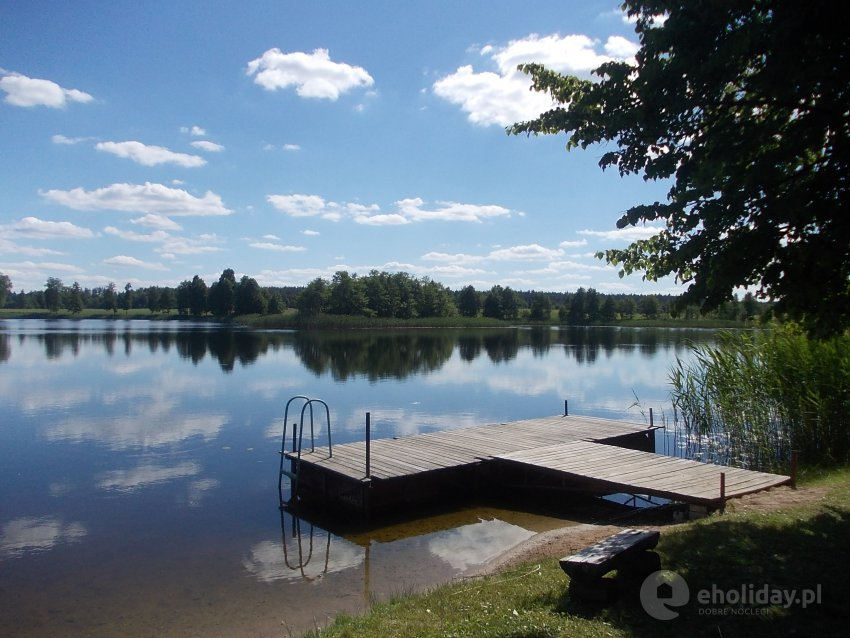
\includegraphics[scale=0.15]{giby1.jpeg}
\column{0.4\textwidth}
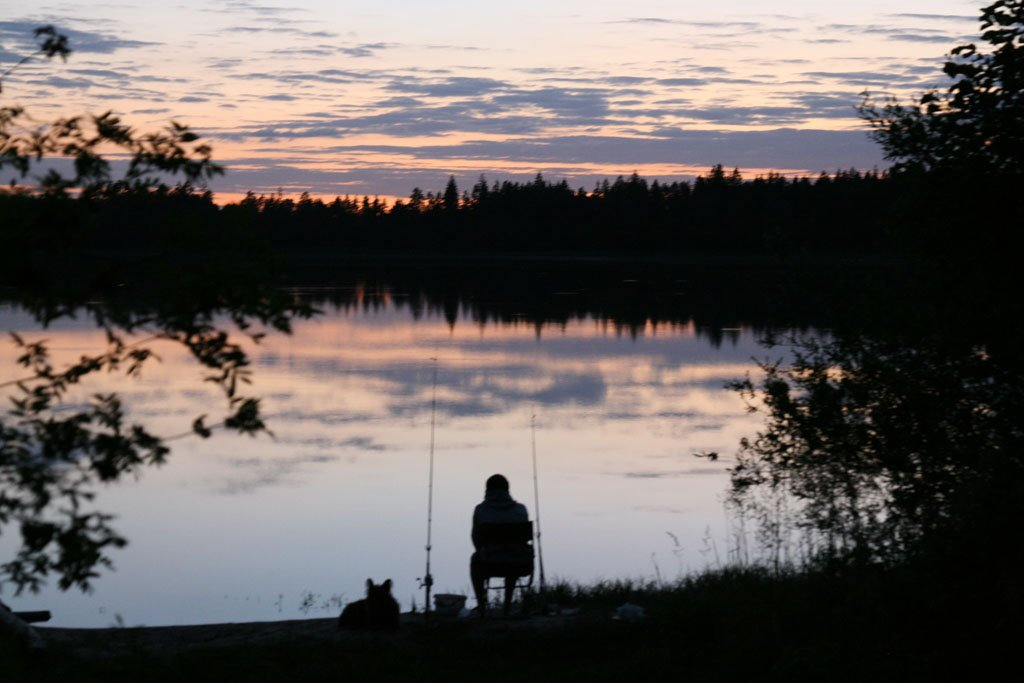
\includegraphics[scale=0.14]{giby2.jpg}
\end{columns}
}
\frame
{
\begin{alertblock}
{POSŁUCHAJ!}
Jeszcze nie jesteś pewny czy chcesz odwiedzić nasze strony ?
\end{alertblock}
\frame
\frametitle{powody}
\begin{itemize}
\item Mnóstwo noclegów w atrakcyjnej cenie do wyboru 
\item Plaże,bary,restauracje,hotele 
\item Przepyszne regionalne wyroby 
\end{itemize}}
\frame
{
 \frametitle{Lasy,jeziora,wyspy}
 \begin{block}
 {Obława}
Obława augustowska (obława lipcowa, obława augustowsko-suwalska) była pacyfikacją terenu Puszczy Augustowskiej i jej okolic przeprowadzoną w lipcu 1945 r. przez jednostki Wojsk Wewnętrznych NKWD i Armii Czerwonej przy pomocy oddziałów WP oraz miejscowych funkcjonariuszy UB i MO.
 Właśnie w Gibach usytuowano w 1991 r. pomnik poświęcony ofiarom obławy. Więcej pod adresem:www.slady.ipn.gov.pl/sz/projekt-naukowo-badawc/wojewodztwo-podlaskie/giby/7751,Oblawa-augustowska-1945.html
\end{block}}
\frame
{
\begin{figure}[here]
\begin{center}
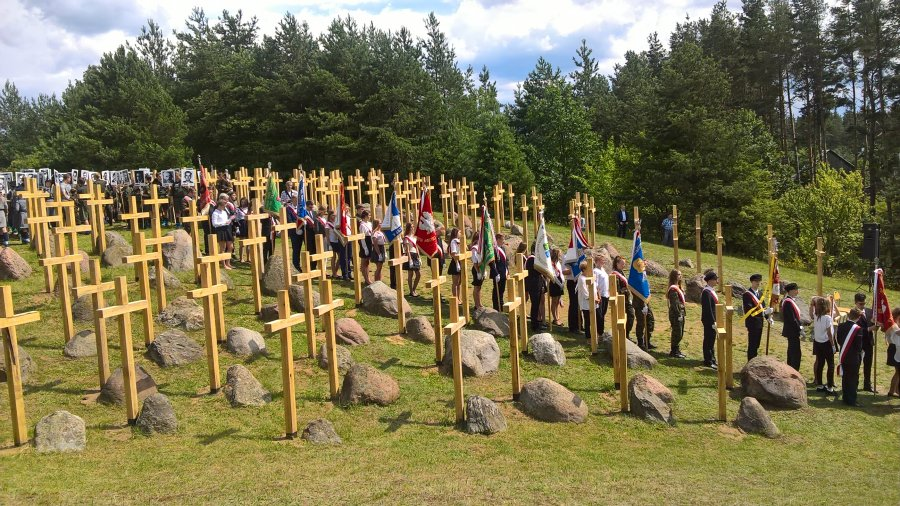
\includegraphics[scale=0.5]{giby3.jpg}
\end{center}
\end{figure}
}
\frame
{
\begin{figure}[here]
\begin{center}
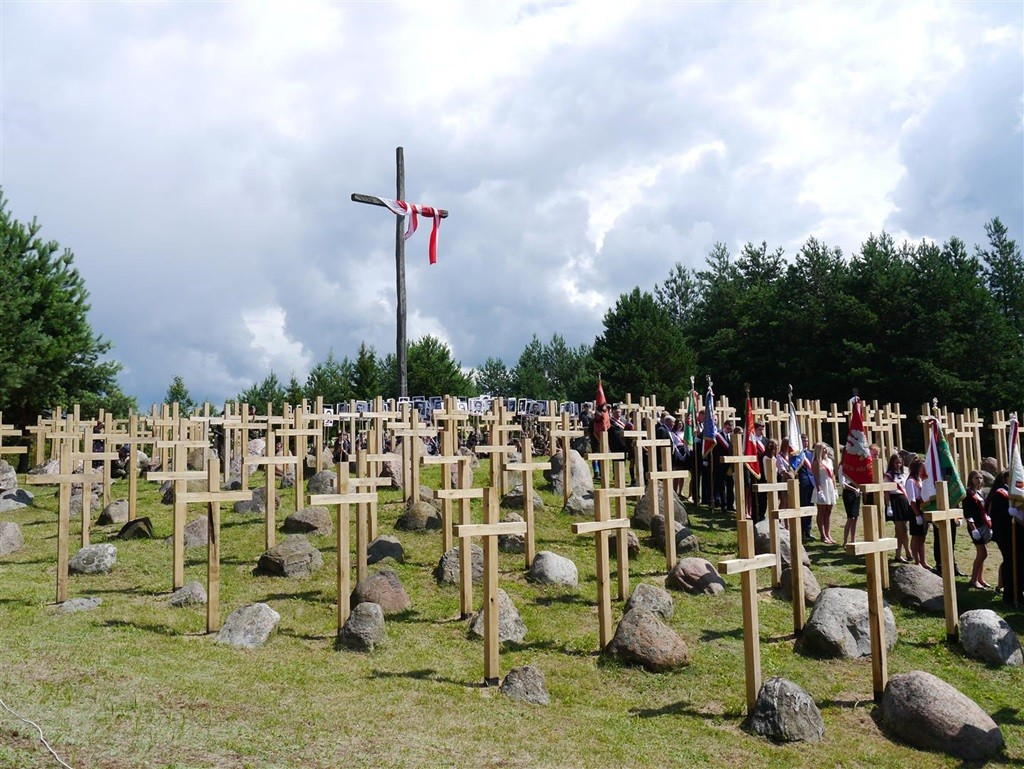
\includegraphics[scale=0.3]{giby4.jpg}
\end{center}
\end{figure}
}
\frame
{
\frametitle{Pobliskie atrakcje,ciekawe miejscowości}
Pomijając już fakt, że w okolicy znajduje się mnóstwo łowisk i plaż, są też inne ciekawe miejsca.
W Kuklach znajduje się jedyna chyba taka `` Wioska Smerfów'', w której możemy wynająć domek wyglądający jak ten w smerfach. Choć na zewnątrz to tylko glina w środku czeka nas wysoki standard. Nie daleko znajduje się też Augustów, piękna miejscowość turystyczna w której podczas wakacji znajdziemy mnóstwo atrakcji niemal każdego dnia}
\frame
{
\begin{figure}[here]
\begin{center}
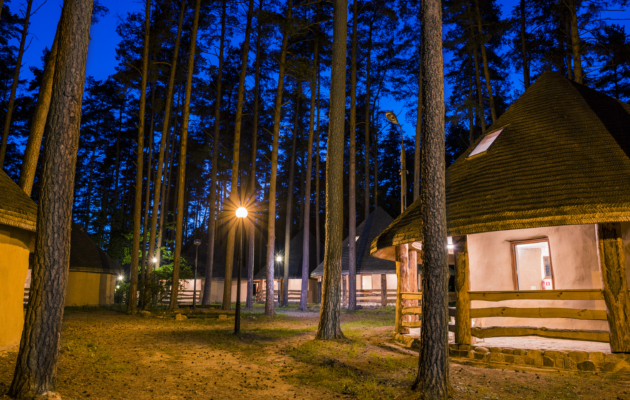
\includegraphics[scale=1]{giby5.jpg}
\end{center}
\end{figure}
}
\frame
{
\begin{figure}[here]
\begin{center}
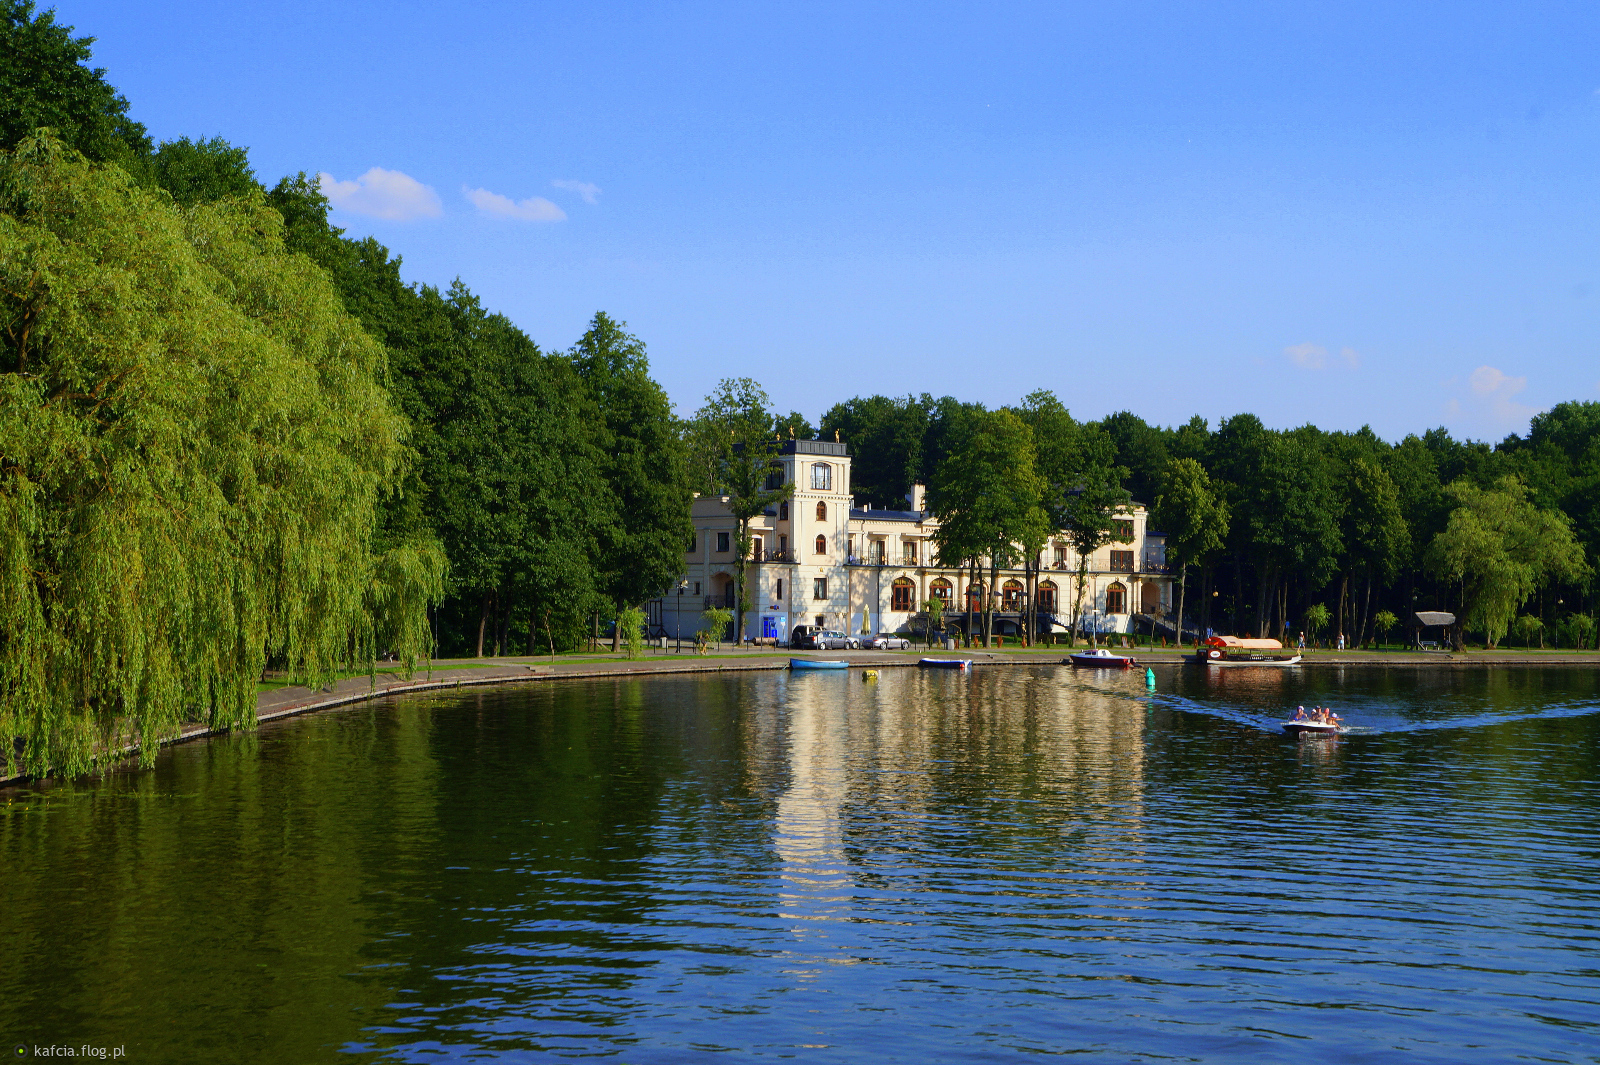
\includegraphics[scale=1]{august.jpg}
\end{center}
\end{figure}
}
\end{document}

